\documentclass[runningheads,a4paper]{llncs}
\usepackage{mathtools}
\usepackage{graphicx}

\begin{document}
\title{Automata-theoretic Modeling of Distributed Controllers}
\maketitle


The problem we are interested in is broadly as follows. We are given a set
of control applications, each of which is partitioned into a set of tasks. Each of
these tasks are mapped onto different processors. The processors and hence the
tasks communicate over one or more shared buses. The tasks on each processor
are scheduled using a given scheduling policy. The messages on the shared buses
are also scheduled using a given arbitration policy.

We will use the term platform to refer to such an (i) architecture (i.e., the
processors, their connections via buses, and the mapping of tasks on the pro-
cessors and messages on the buses), as well as (ii) the different scheduling and
arbitration policies used.

Now let us consider two tasks $T_1$ and $T_2$ belonging to the same control
application, with $T_1$ and $T_2$ mapped onto different processors. $T_1$ for example
can be a sensor task and T 2 can be a controller task. T 1 and T 2 communicate
via a message stream $M$, consisting of an infinite sequence of message instances
$m_1$, $m_2$ , . . .. Assuming that $T_1$ senses at a constant periodic rate, the delay
from the instant $T_1$ senses to the time $T_2$ receives the sample depends on the

(i) processing delay suffered by $T_1$ because of the other tasks scheduled on the
same processor, and 

(ii) the delay suffered by the messages sent by $T_1$ because
of the other messages scheduled on the shared bus.

For the moment, let us focus only on the message delays. The extension to
account for delays arising from the task scheduling can be handled later in a
similar fashion.

The delays suffered by the messages will influence the performance of the
control application. Since these delays will depend on the platform (e.g., the
mapping of the tasks, scheduling policies, etc.), certain choices of the platform
will result in acceptable control performance and others will not.

In this setup, we are interested in answering questions of the form:
\begin{itemize}
 \item Given a platform and a set of control applications, does the platform meet
the control performance requirements of the different applications?
 \item  Given a set of control applications, can we synthesize a platform (or a part
of it, e.g., the scheduling policy on a bus) to meet the control performance
requirements of the different applications?
\end{itemize}




\textbf{Problem 1:}

Let us assume that the controller has been designed (or optimized) with the
assumption that the delays suffered by messages is bounded by one sampling
period (i.e., this is the deadline). If certain message instances, e.g., m i , m j ,
m k , . . ., miss this deadline then this will negatively impact control performance.

However, if not too many messages miss their deadlines then the control performance
might be within the acceptable limit.
In this problem, we will specifically consider deadline misses of the following
form:
every invalid message $m_i$ is followed by at least $k$ valid messages
$m_{i+1}$, \dots $m_{i+k}$,
where a message that misses its deadline is referred to as an invalid message
and one that meets its deadline is referred to as an valid message.
Let us assume that for a certain k a given control performance requirement
is satisfied (details on this may be found in [?]).
Question (Verification): Is this $k$ satisfied by the platform?

To answer this question, we can start with a simple setup with only two processors
communicating via a bus. The bus implements a given scheduling policy
(e.g., TDMA, fixed priority, or any other), with messages from the application
at hand being scheduled with messages from other applications that are not being 
analyzed. We would like to apply model checking techniques to answer if the
given k is satisfied by the bus scheduling policy and messages to be scheduled.
This setup can then be extended to consider not only the schedule on the
bus, but also the scheduling policies on the processors.
Question (Synthesis): For a given k, can we synthesize a bus schedule such
that the platform satisfies this k?
Again, this synthesis problem may be extended to consider not only bus
schedules but also the processor schedules.

\textbf{Motivating Example:}

\begin{figure}
\begin{center}
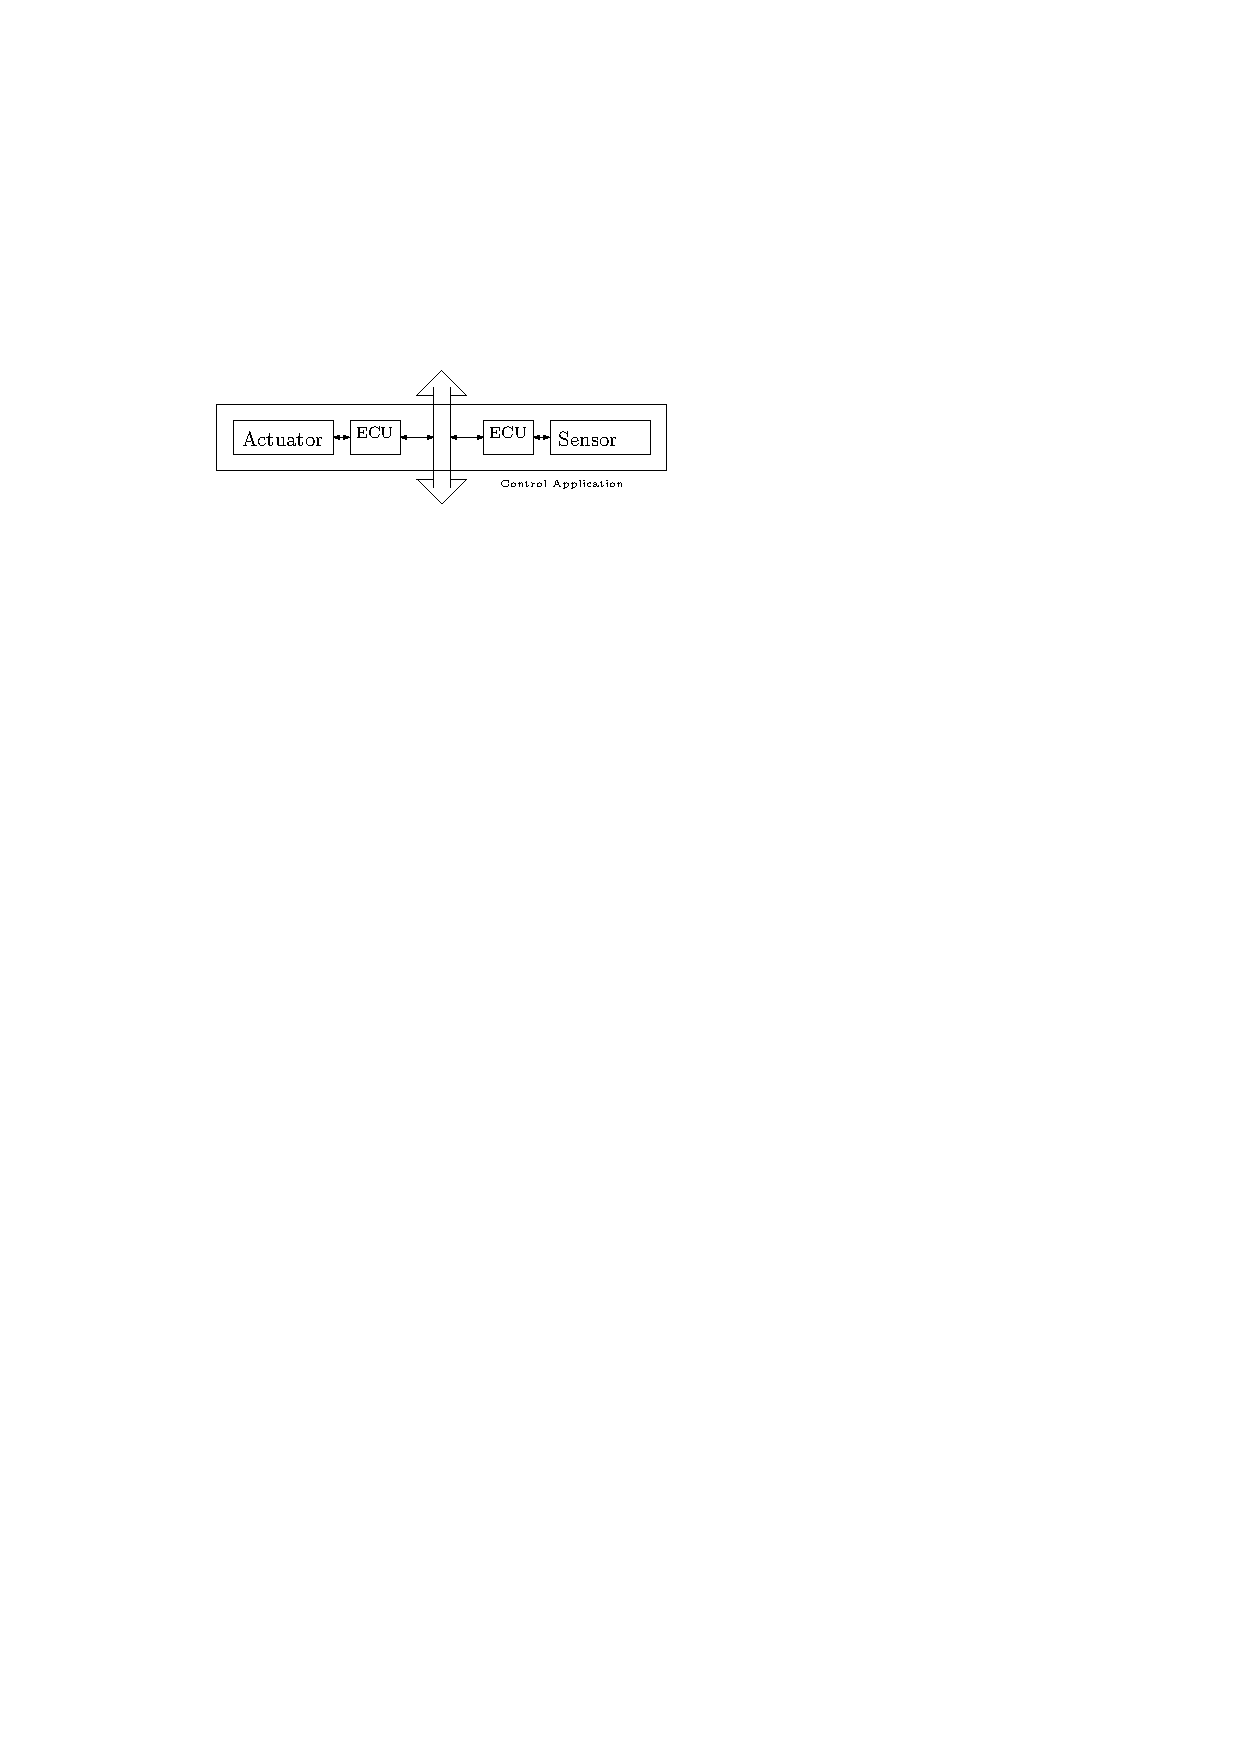
\includegraphics[width = 80mm]{system_block_diagram.pdf}
\end{center}
\caption{System Block Diagram}
\label{block_dig}
\end{figure}

The diagram of the distributed platform is given in Fig.\ref{block_dig}.
In the diagram a control application is divided into two tasks, a sensor task $T_s$ and 
an actuator task $T_a$. These tasks run on two different processors and
uses a common shared bus. A bus schedule is there to schedule messages on the bus.
When sender generates a message, it waits for the bus scheduler to get the bus
access and when bus scheduler allots bus to the message it gets transmitted to
the receiver's processor to be accessed by the receiver. Say at a particular period  
$p$, $T_a$ sends message $m_a$ to the bus and receive feedback message $m_s$ and $T_s$
accepts message $m_a$ and sends feedback message $m_s$. The timing diagram is given in Fig.\ref{tim_dig}

\begin{figure}
\begin{center}
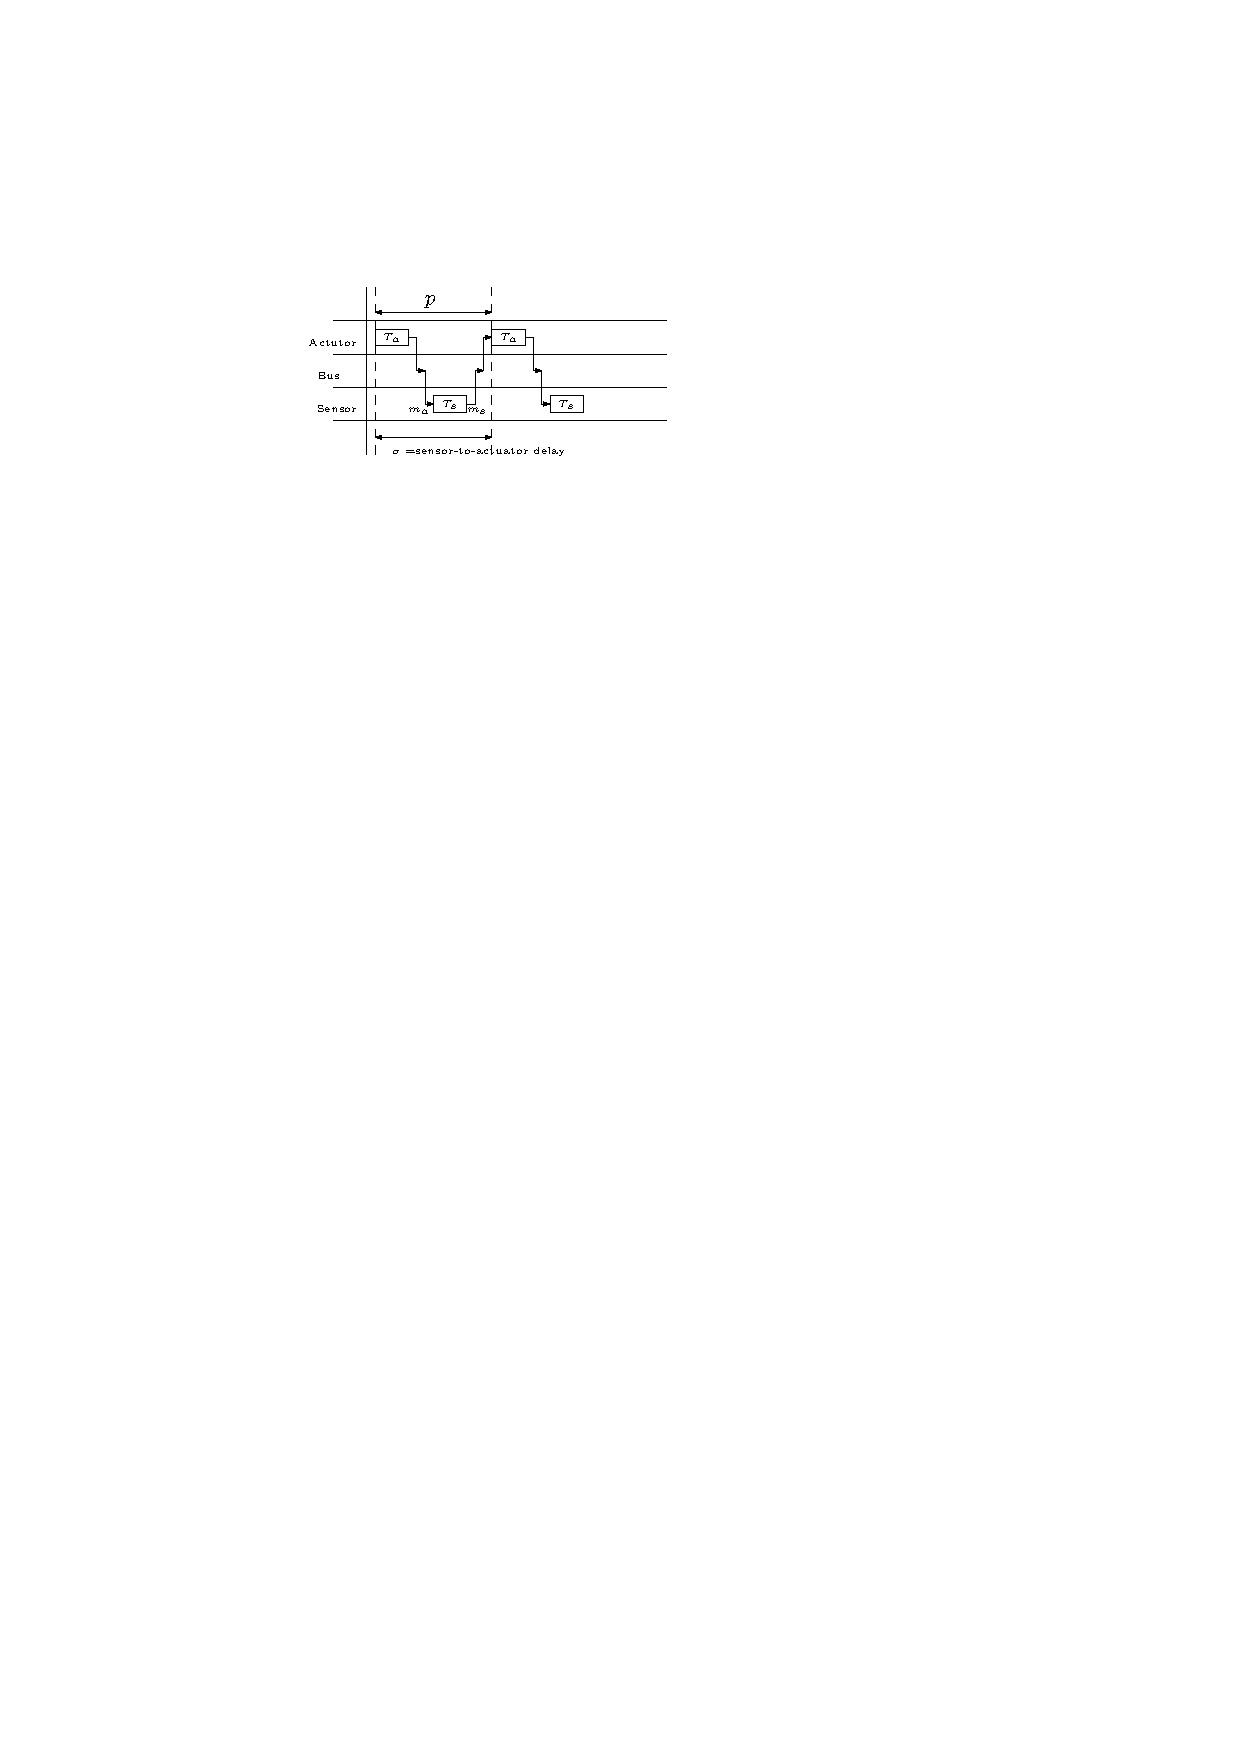
\includegraphics[width=75mm]{timing_diagram_deadline_cosntraint.pdf}
\end{center}
\caption{Timing diagram}
\label{tim_dig}
\end{figure}


The time interval between the sending message and receiving message is the
sensor-to-actuator delay denoted by $\sigma$. According to the timing diagram,
the sensor-to-actuator delay can be measured by total time needed by $T_a$
to send $m_a$ and getting feedback message $m_s$, which is some function of $m_a$,
i.e $m_s = f(m_a)$. 

From the timing diagram we can understand that $\sigma > 0$ and $\lceil{h|\sigma}\rceil >= 1$
should be true always. Such kind of constraint are common in computational process and 
control algorithms where they share a common bus in a distributed environment.


\begin{figure}
\begin{center}
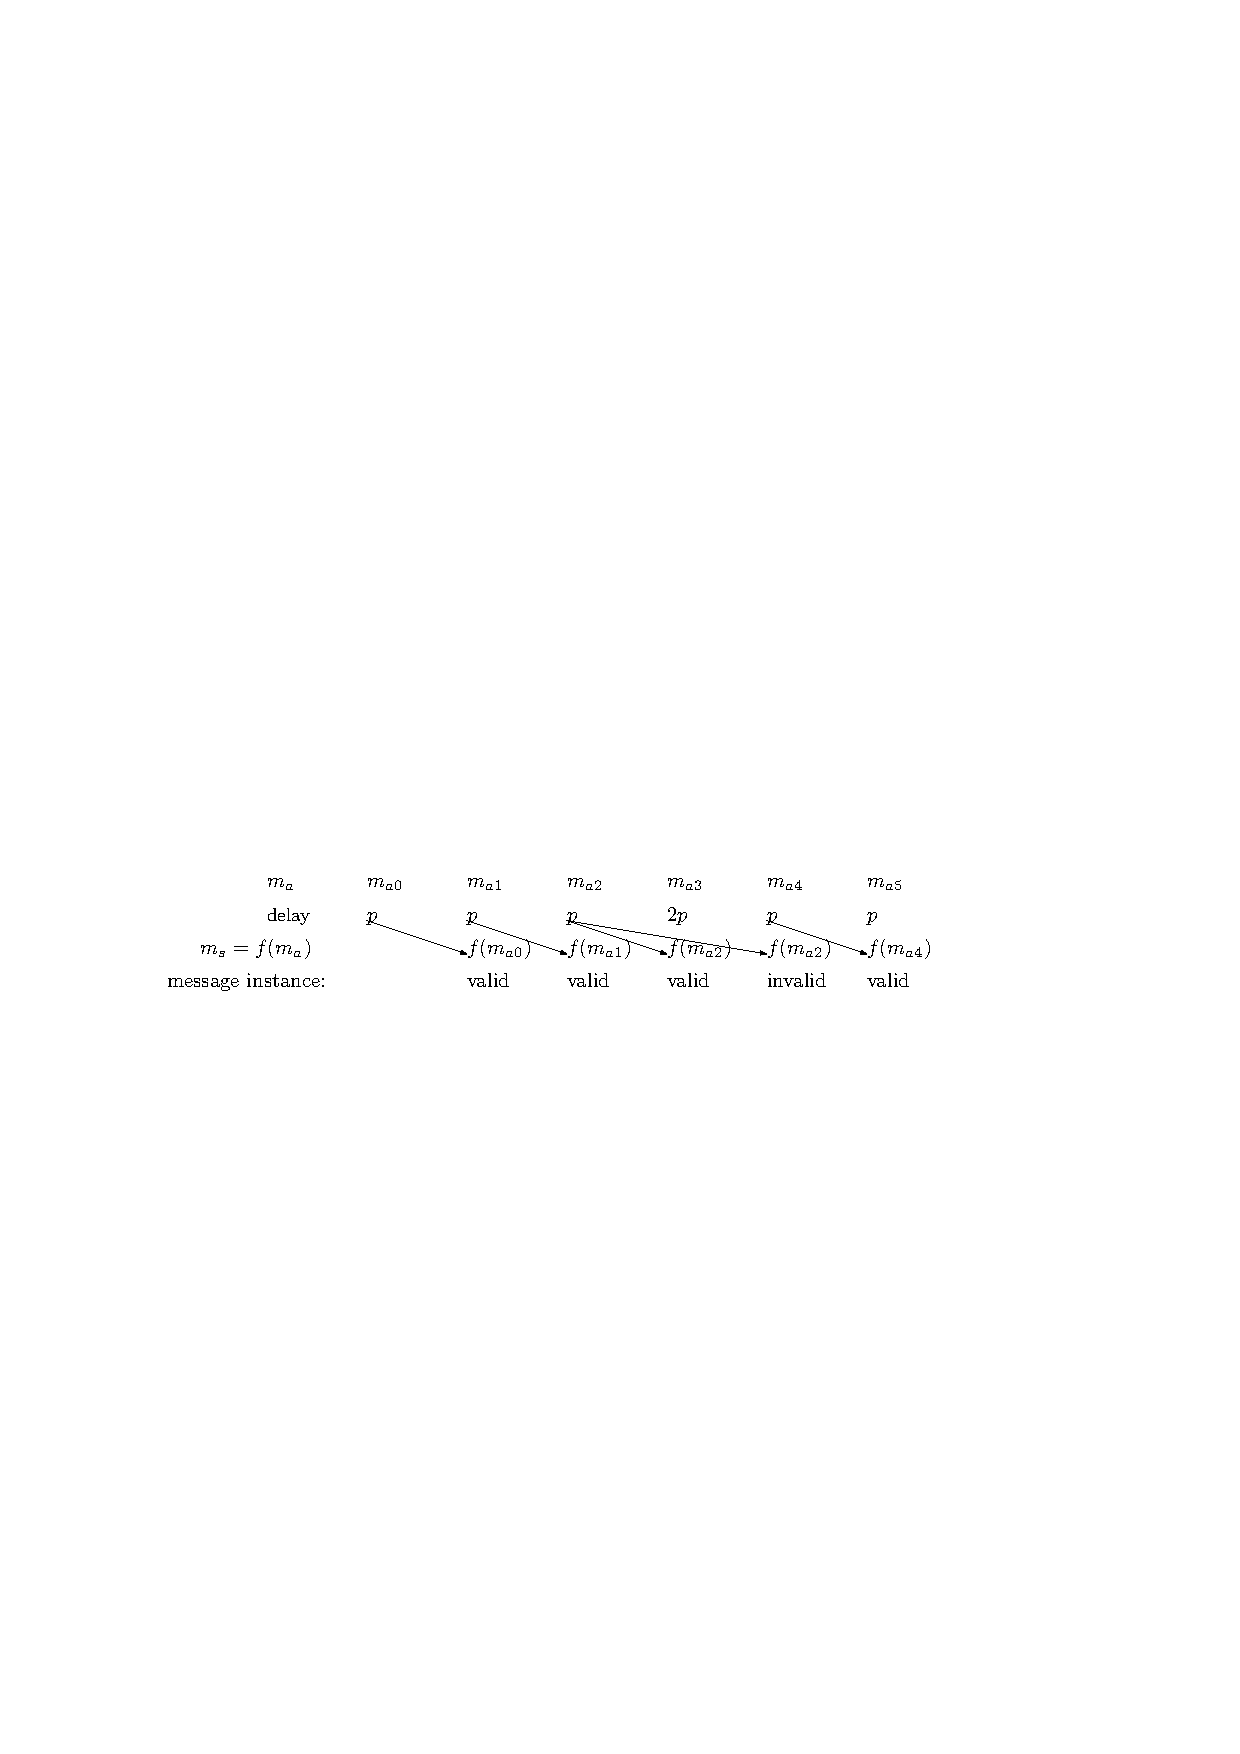
\includegraphics[width = 100mm]{timing_diagram_delay_cosntraint.pdf}
\end{center}
\caption{Timing diagram showing valid invalid sequence}
\label{tim_dig_delay}
\end{figure}

\begin{figure}
\begin{center}
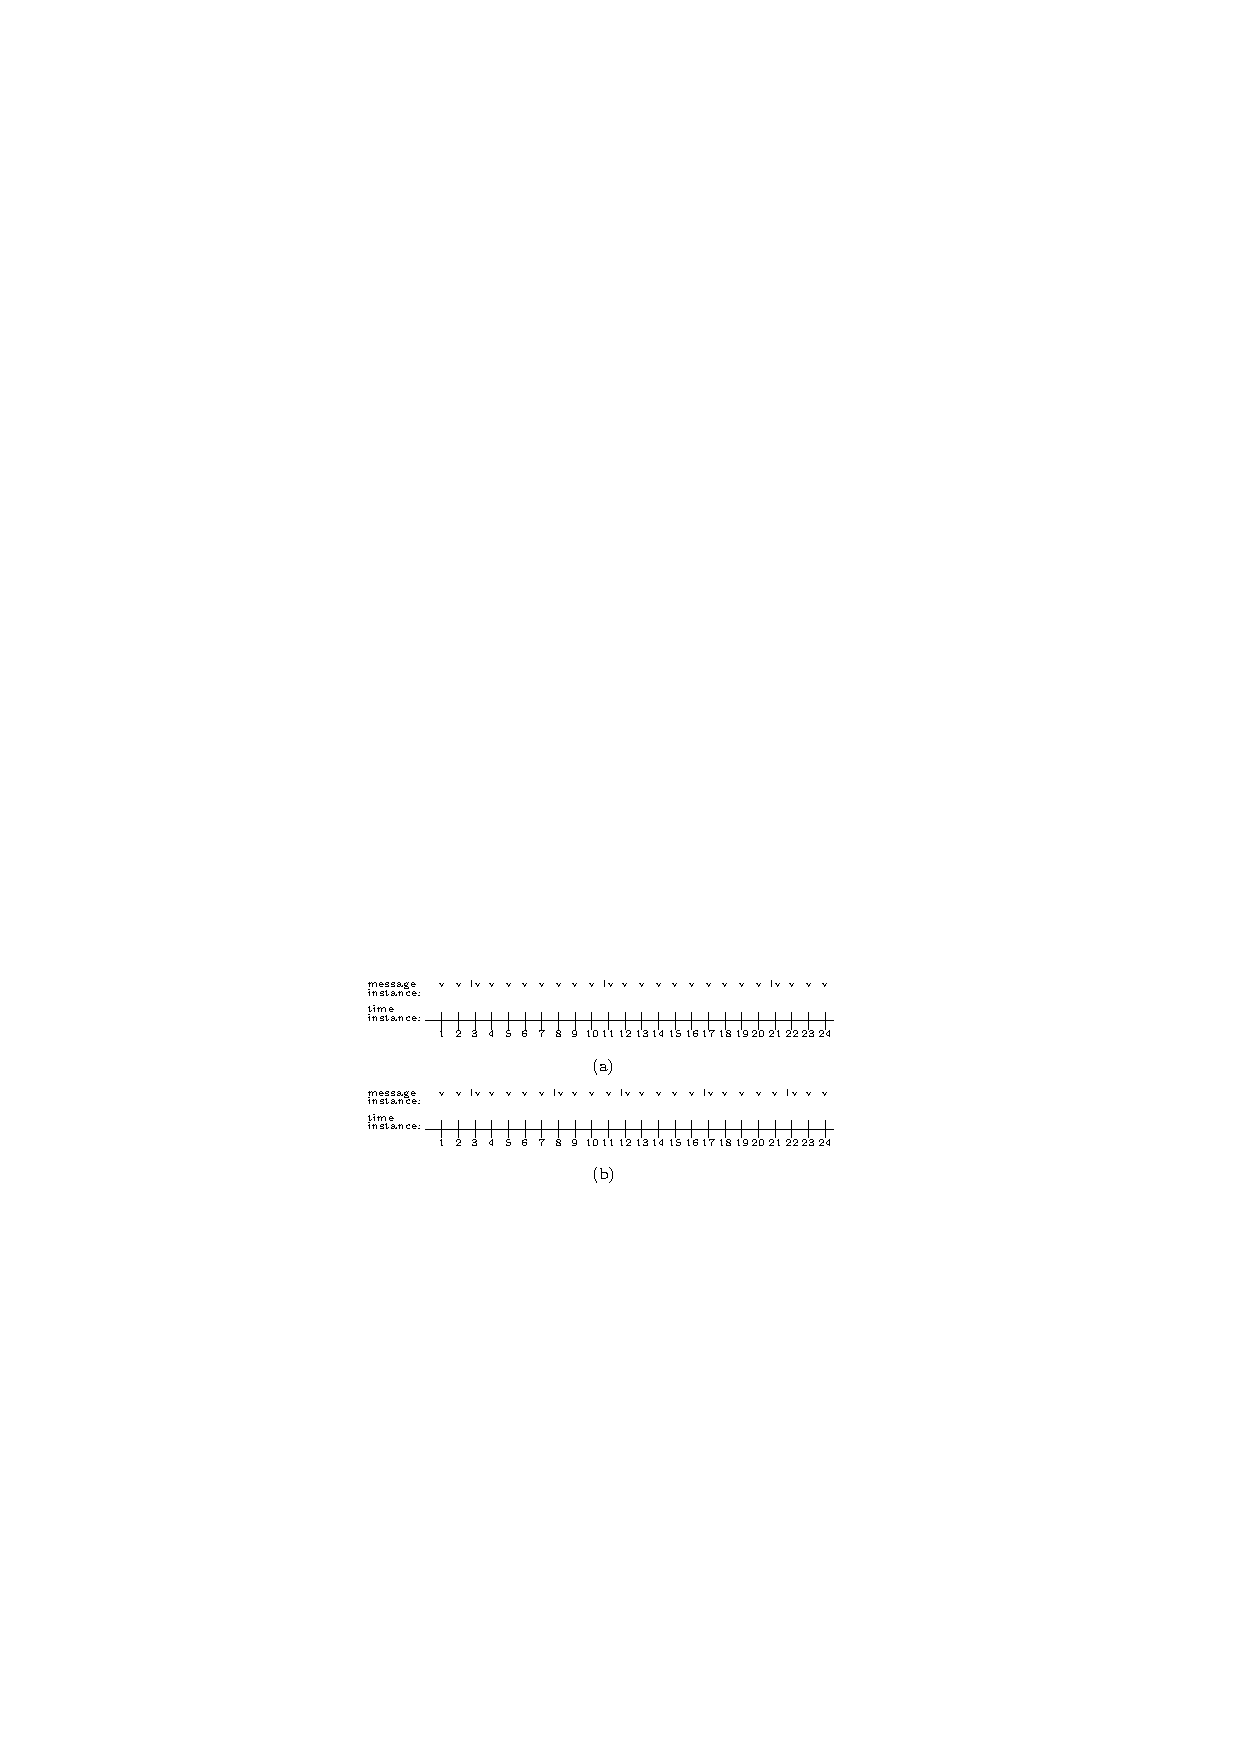
\includegraphics[width = 120mm]{valid_invalid.pdf}
\end{center}
\caption{Valid-Invalid messages from infinite sequence}
\label{tim_dig_cons}
\end{figure}


If a message is delivered within the particular period $p$ then it is called valid message but
if it is not delivered within $p$ period it becomes invalid. In the Fig.\ref{tim_dig_delay} we see that message
instance $m_{a3}$ requires $2p$ time period, so it does not get delivered within $p$ period and 
$m_{s2} = f(m_{a2})$ is delivered again which is now invalid.

In this problem model we are trying to demonstrate a system where an invalid message should 
followed by at least k valid messages. In Fig.\ref{tim_dig_cons}, we depicted the occurrence of invalid messages.
in Fig.\ref{tim_dig_cons}(a), invalid messages occurred after at least $k=6$ intervals but 
in Fig.\ref{tim_dig_cons}(b), invalid
messages occurred more frequently which will negatively impact the control performance.









\textbf{Problem 2:}

We may extend the above problem with more general patterns of deadline
misses. Such patterns may be represented as infinite strings over the alphabet {0, 1},
such as $111011101110 \dots$, where a $1$ denotes that the corresponding
message instance meets its deadline constraint and $0$ denotes that the corresponding 
message instance misses its deadline constraint.

Based on a control-theoretic analysis, we can compute the set of all possible
such infinite strings which denote deadline miss patterns corresponding to which
given control performance constraints are satisfied. Let such a set of strings be
given by the language $L_{controller}$.

Similarly, given a platform, as in the case of Problem 1, let infinite strings
over the alphabet ${0, 1}$ denote transmission times of message instances over a
shared communication bus. Here, again, $1$ denotes that the corresponding message
instance meets its deadline constraint and $0$ denotes that the corresponding
message instance misses its deadline constraint. Such strings may be computed
using standard schedulability analysis techniques or model checking techniques
that analyze the platform (or scheduling policy) at hand. Let the set of such
strings be denoted by the language $L_{platform}$ .
Clearly, if $L_{platform} \subseteq L_{controller}$ then the control performance requirements
are satisfied when the control application is implemented on the platform in a
distributed fashion.
Again, we may ask different questions in this setup.


Question (Verification): Given control performance constraints for each 
controller, and a platform, are all the constraints satisfied?

Question (Synthesis): Given control performance constraints for each controller,
and a mapping of the control tasks on a distributed architecture, synthesize
bus or/and processor schedules such that the performance constraints
are satisfied.

\begin{figure}
\begin{center}
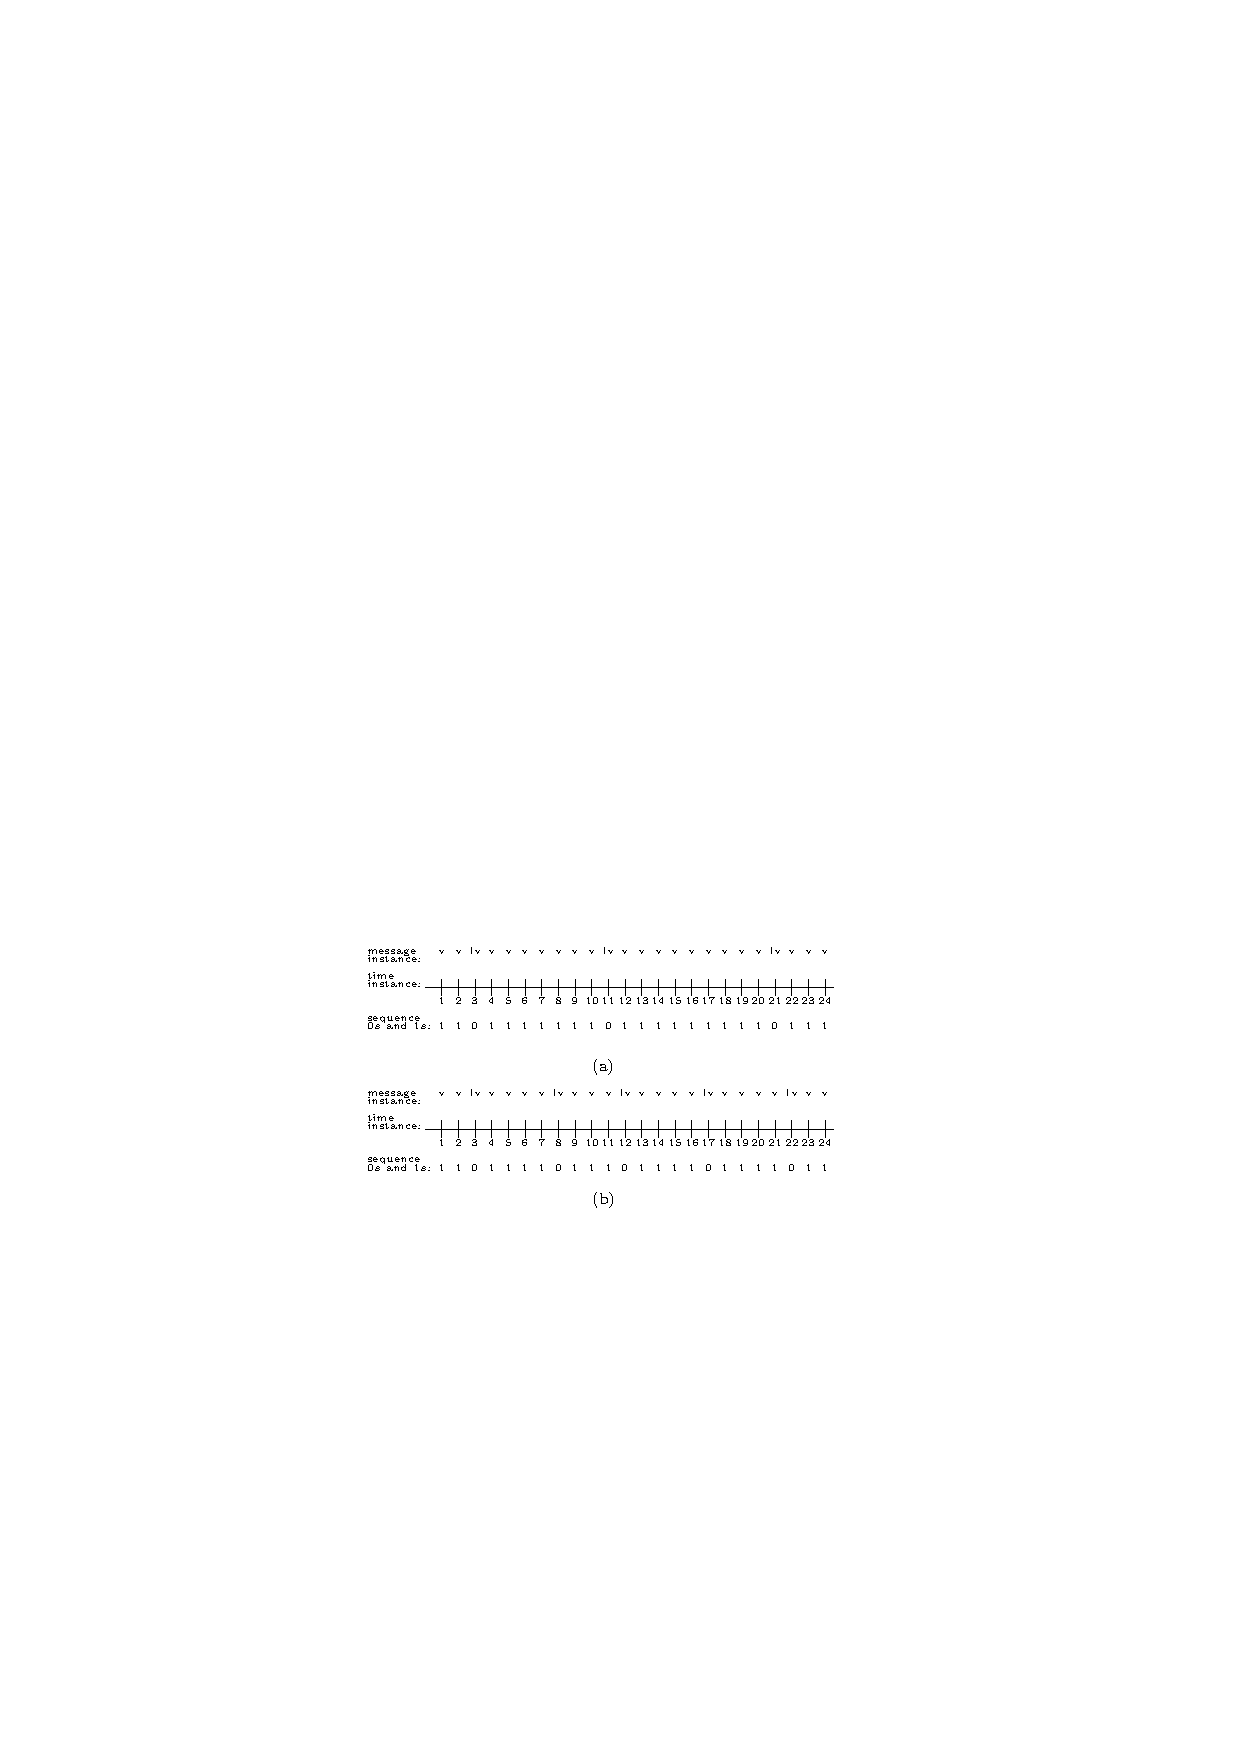
\includegraphics[width = 120mm]{vali_invalid_0_1.pdf}
\end{center}
\caption{Timing diagram}
\label{tim_dig_01}
\end{figure}

\textbf{Motivating Example:}
Let us consider the motivating example for Problem1. From the diagram Fig.\ref{tim_dig}, we  are representing
such valid-invalid sequence into streams of $0$ and $1$ where $1s$ represent valid massage
and $0s$ represent invalid messages. We considered that an invalid
message should be followed by at lest $k = 6$ valid messages. Now if we consider a $10$
length timing sample then possible satisfied combinations will be denoted by $L_{controller}
= \{ 0111111011, 1011111101,$ 

$1101111110, 0111111101, 0111111110, 1011111110, 0111111111, 1011111111, 1101111111,$ 

$1110111111, 1111011111, 1111101111, 11111101111, 11111110111, 11111111011, 1111111110\}$. Now if any $10$ 
length sequence satisfying the above condition will be any of the above mentioned sequence.
Any sequence other that these sequences will be vulnerable for the system.

In the Fig.\ref{tim_dig_01} the valid-invalid sequence is represented by streams of $0s$ and $1s$.
Now  we can say, that the sequence represented in Fig.\ref{tim_dig_01}(a) matches one
of the sequence but the sequence represented by Fig.\ref{tim_dig_01}(b) cannot match any of the 
satisfied sets of sequence. From Fig.\ref{tim_dig_01}(a), if we consider a $10$ length sequence
arbitrarily, say 7th slot to 16th slot. Here, $L_{platform} = 1111011111$ which is one of the
sequence present in $L_{controller}$, i.e, $L_{platform} \subseteq L_{controller}$. We can take
any of the $10$ length sequence and check the $L_{controller}$ set, then if the sequence is obeying
our satisfying constraint, then all of them will belong to that $L_{controller}$. But if it is not satisfying
like Fig.\ref{tim_dig_01}(b), we will get such sequence which does not belong to $L_{controller}$.


Solution Approach:
Instead of considering the full infinite sequence we can consider a window of size $w > (k + k/2)$. 
Because generating all possible sequence for infinite sequence will be itself a huge task.

For a given platform, if we have the satisfying constraint then we can get all of the valid
combinations of length $W$ satisfying the given constraint. If this window now passes through 
the infinite sequence and check whether it belongs to the valid set i.e, $L_{controller}$ , if 
we get valid sequence repeatedly then the system is safe. But if we get no match frequently, then 
from the safety property we can call the sequence as bad prefix.




Related work: Language/automata-theoretic formulations of control perfor-
mence metrics have been studied in [?, ?]. The problem of characterizing dead-
line miss patterns under which control performence metrics like asymptotic sta-
bility is satisfied has been studied in [?]. Here, such a characterization has been
restricted to a ratio between the number of messages that meet their deadlines
to the number of messages that miss their deadlines. The problem we have
listed above will generalize such a result.

\end{document}